\chapter{Experimental Results}\label{ch:results}

\begin{flushright}
	\emph{\lq\lq A victory is twice itself when the achiever brings home full numbers.\rq\rq \\
		       \emph{Much ado about nothing}, Leonato, scene 1.}
\end{flushright}

\vspace{0.6cm}

In {\bf chapter \ref{ch:introduction}} the concept of log-composition is introduced, with its implications in medical imaging, as in diffeomorphic registration and in the computation of the logarithm in the log-Euclidean framework. 
{\bf Chapter \ref{ch:tools}} is devoted to the introduction of the underpinning mathematical theory. Here are presented three numerical methods for the computation of the log-composition:
\begin{enumerate}
	\item Truncated BCH formula of degree $k=1,2,3$ - equation \ref{eq:bch_definition}.
	\item Taylor expansion - equation \ref{eq:taylor}.
	\item Parallel transport - equation \ref{eq:parallel_transport}.
\end{enumerate}
To evaluate their performance, two groups of transformations are presented in {\bf chapter \ref{ch:spatial_transformations}} with respective numerical methods for their log-composition:
\begin{enumerate}
	\item The finite dimensional Lie group of euclidean transformation SE(2) - section \ref{se:rigid_body_transformations}
	\item The infinite dimensional Lie group diffeomorphisms, set of images of SVF through the Lie exponential map - section \ref{se:svf}
\end{enumerate}

The computation of the Lie logarithm as an important piece in the jigsaw puzzle of the log-euclidean framework is presented in {\bf chapter \ref{ch:log_algorithm}} within the log-algorithm \cite{Bossa:08}. 
The numerical methods tailored for the computation of the log-algorithm here proposed are
\begin{enumerate}
	\item Truncated BCH formula of degree $k=1,2,3$ - equation \ref{eq:bossa_bch_strat}.
	\item Parallel transport - equation \ref{eq:bossa_parallel_strategy}.
	\item Symmetric parallel transport - equation \ref{eq:bossa_symmetric}.
\end{enumerate}

In this last chapter we will compare the results of the numerical methods presented so far.
The performance of the log-composition with each of the presented methods, applied to the groups of transformations $SE(2)$ and diffeomorphisms parametrized by SVF, is evaluated over synthetic datasets.\\
Following results are computed using a software written in Python (available on gitlab at ... add ref).

% % % % % % % % % % % % % % % % % % % % % % % % % % % % % % % % % % % % % %
% % % % % % % % % % % % % % % % % % % % % % % % % % % % % % % % % % % % % % 
% % % % % % % % % % % % % % % % % % % % % % % % % % % % % % % % % % % % % % 
\section{Log-composition for $\mathfrak{se}(2)$}



% % % % % % % % % % % % % % % % % % % % % % % % % % % % % % % % % % % % % %
% % % % % % % % % % % % % % % % % % % % % % % % % % % % % % % % % % % % % % 
\subsection{Methods}

A set of $500$ transformations in $\mathfrak{se}(2)$ are sampled with a randomizer. Whereas the Frobenius norm of the matrix representation of $SE(2)$ is not proportional to the rotation angle $\theta$, in $\mathfrak{se}(2)$ it is
\begin{align*}
\euclideanMetric{(\theta,dt_{x},dt_{y})}_{\text{fro}} = \sqrt{2\theta^{2} + dt_{x}^2 + dt_{y}^2} 
\end{align*}




% % % % % % % % % % % % % % % % % % % % % % % % % % % % % % % % % % % % % %
% % % % % % % % % % % % % % % % % % % % % % % % % % % % % % % % % % % % % % 
\subsection{Results}


\begin{figure}[!ht]
	%\centering
	\hspace{-1cm}
	\includegraphics[scale=0.65]{figures/se2_four_BCH.png}
	\caption{Log composition in $\mathfrak{se}(2)$. Comparisons between BCH methods. TODO}
	\label{fig:se2_four_BCH}
\end{figure}

\begin{figure}[!ht]
	%\centering
	\hspace{-2cm}
	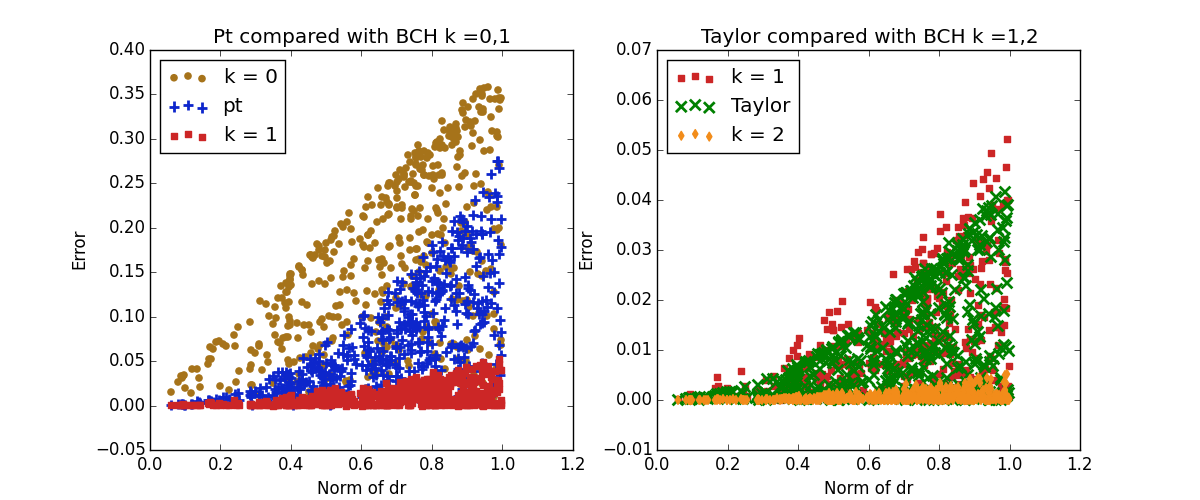
\includegraphics[scale=0.6]{figures/se2_pt_taylor.png}
	\caption{Log composition in $\mathfrak{se}(2)$. Comparisons between Parallel Transport method and Taylor method. TODO}
	\label{fig:se2_pt_taylor}
\end{figure}


\begin{figure}[!ht]
	\hspace{-2cm}
	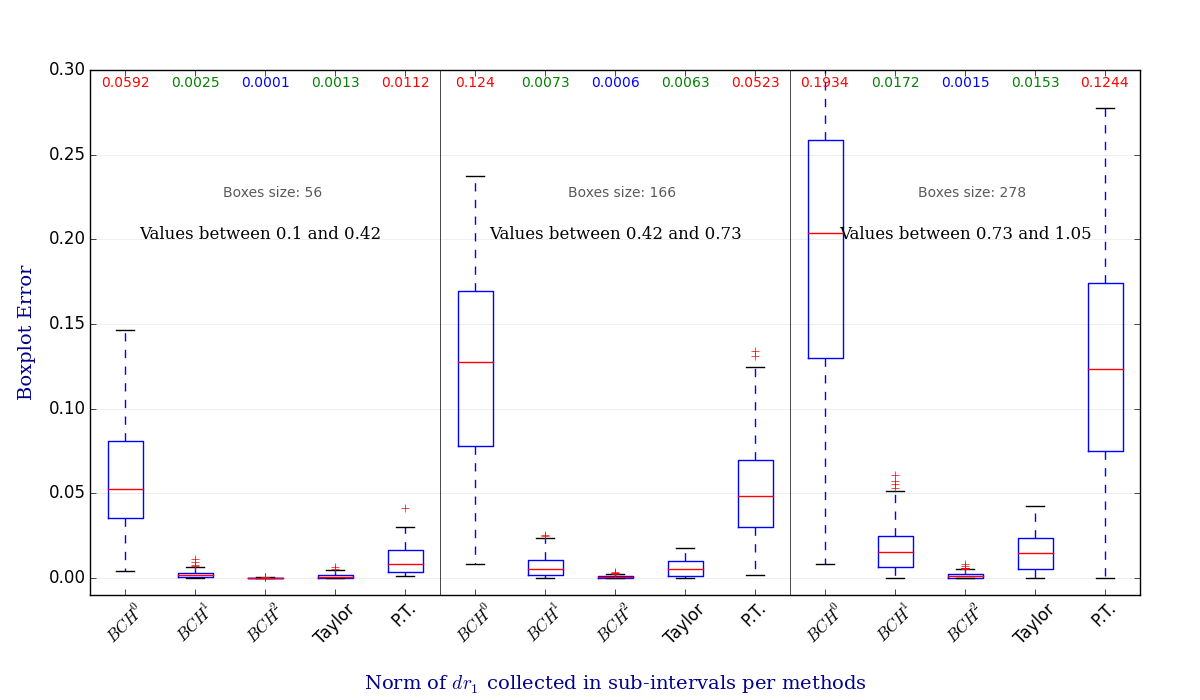
\includegraphics[scale=0.75]{figures/se2_boxplot.png}
	\caption{Log composition in $\mathfrak{se}(2)$. comparisons between all the methods. TODO}
	\label{fig:se2_boxplot}
\end{figure}


% % % % % % % % % % % % % % % % % % % % % % % % % % % % % % % % % % % % % %
% % % % % % % % % % % % % % % % % % % % % % % % % % % % % % % % % % % % % % 
\subsection{Empirical Evaluations of Computational Time}


% % % % % % % % % % % % % % % % % % % % % % % % % % % % % % % % % % % % % %
% % % % % % % % % % % % % % % % % % % % % % % % % % % % % % % % % % % % % %
% % % % % % % % % % % % % % % % % % % % % % % % % % % % % % % % % % % % % % 
% % % % % % % % % % % % % % % % % % % % % % % % % % % % % % % % % % % % % % 
\section{Log-composition for SVF}


% % % % % % % % % % % % % % % % % % % % % % % % % % % % % % % % % % % % % %
% % % % % % % % % % % % % % % % % % % % % % % % % % % % % % % % % % % % % % 
\subsection{Methods: random generated SVF, and norm comparisons.}
We created synthetic random matrices in $\mathfrak{se}(2)$. We considered the difference between the log composition computed with the closed form \ref{eq:log_composition_se2_closed_form}. 
A sample of $500$ couples $(dr_0,dr_1)$ of elements in $\mathfrak{se}(2)$ are created, 

norm in the lie algebra

norm in the lie group

\begin{figure}[!ht]
	\hspace{-1.4cm}
	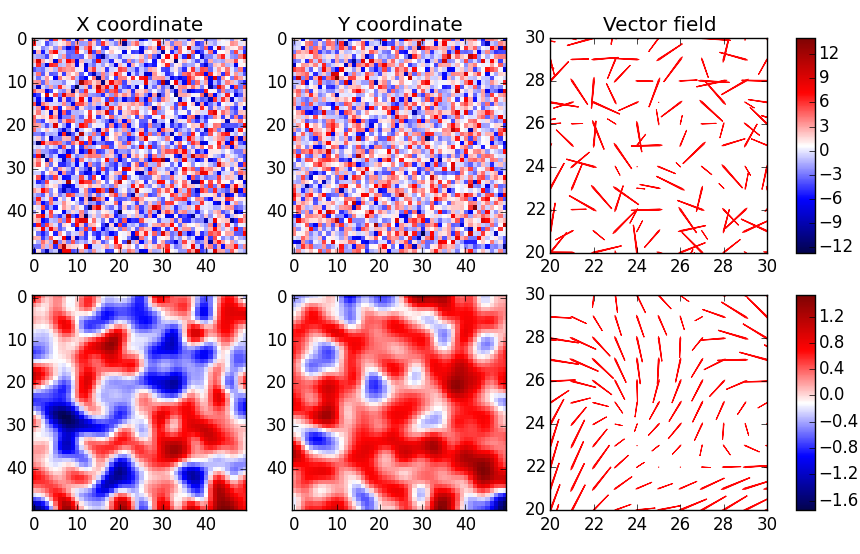
\includegraphics[scale=0.75]{figures/gaussian_smoothing_effect.png}
	\caption{Random generated vector field before and after the Gaussian smoother: in the first row a random generated vector field of dimension $50\times 50 \times 2$ where the value at each pixel are sampled from a random variable with normal distribution of mean $0$ and sigma $4$. The second row shows the same random vector field after a Gaussian smoothing of sigma $2$ (the code is based on the scipy library ndimage.filters.gaussian\textunderscore filter). In the last column shows the quiver of the vector field in the squared subregion of size $10\times 10$ at the point $(20,20)$. From the colorscale it is also possible to see that the values distribution of the filtered image is not anymore symmetric. }
	\label{fig:svf_gaussian_smoothing_effects}
\end{figure}


\begin{figure}[!ht]
	\hspace{-3cm}
	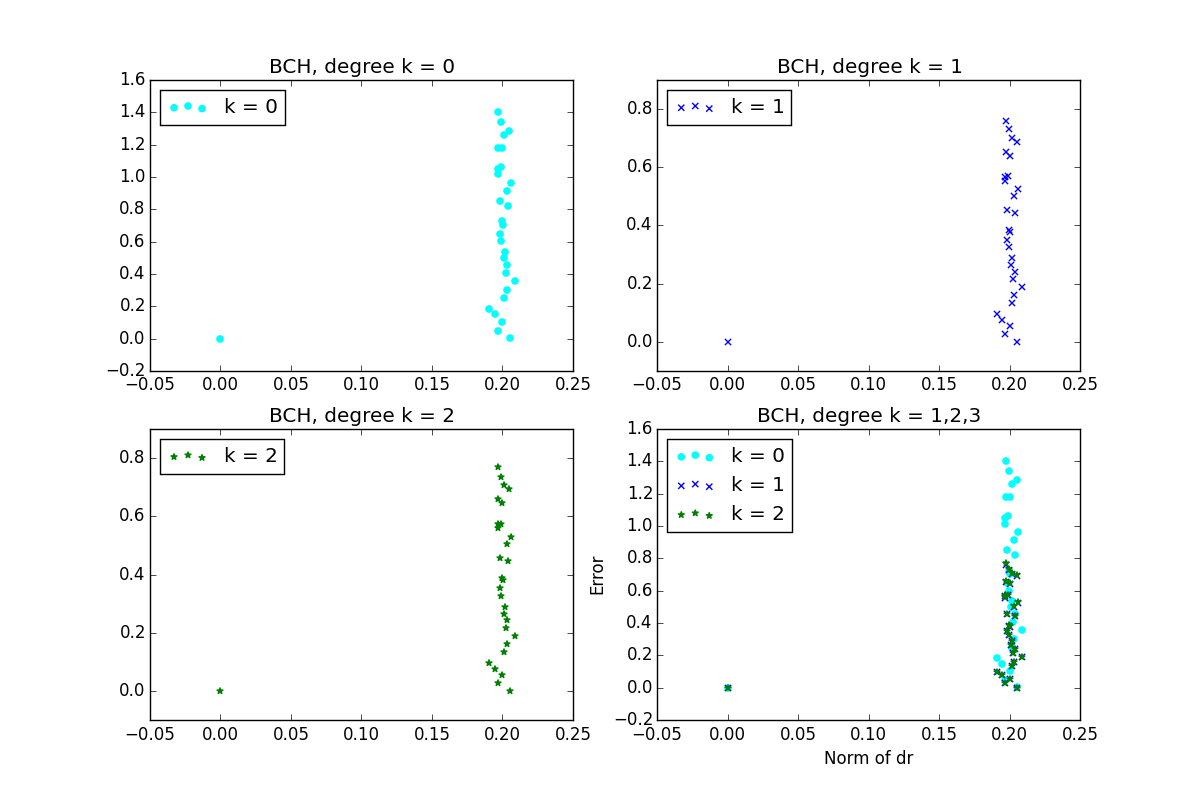
\includegraphics[scale=0.65]{figures/SVF_four_bch.png}
	\caption{Log-composition for SVF computed using numerical methods of truncated BCH of degree 0, 1 and 2. How can we show formally that the error in the case $k=2$ make it not worthed to be computed?}
	\label{fig:SVF_four_bch}
\end{figure}

\begin{figure}[!ht]
	\hspace{-3cm}
	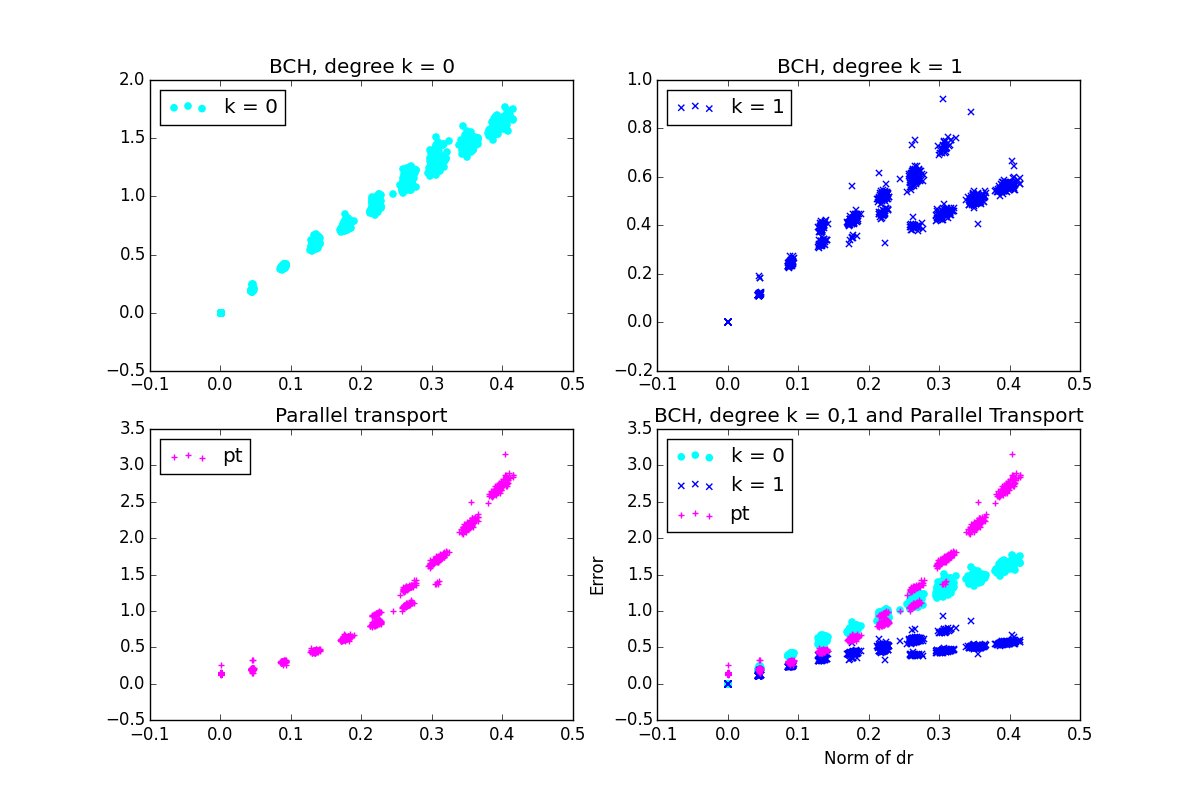
\includegraphics[scale=0.65]{figures/SVF_bch_parallel_transport.png}
	\caption{Log-composition for SVF computed using numerical methods of truncated BCH of degree 0,1 and parallel transport.}
	\label{fig:SVF_bch_parallel_transport}
\end{figure}

\begin{figure}[!ht]
	\hspace{-2cm}
	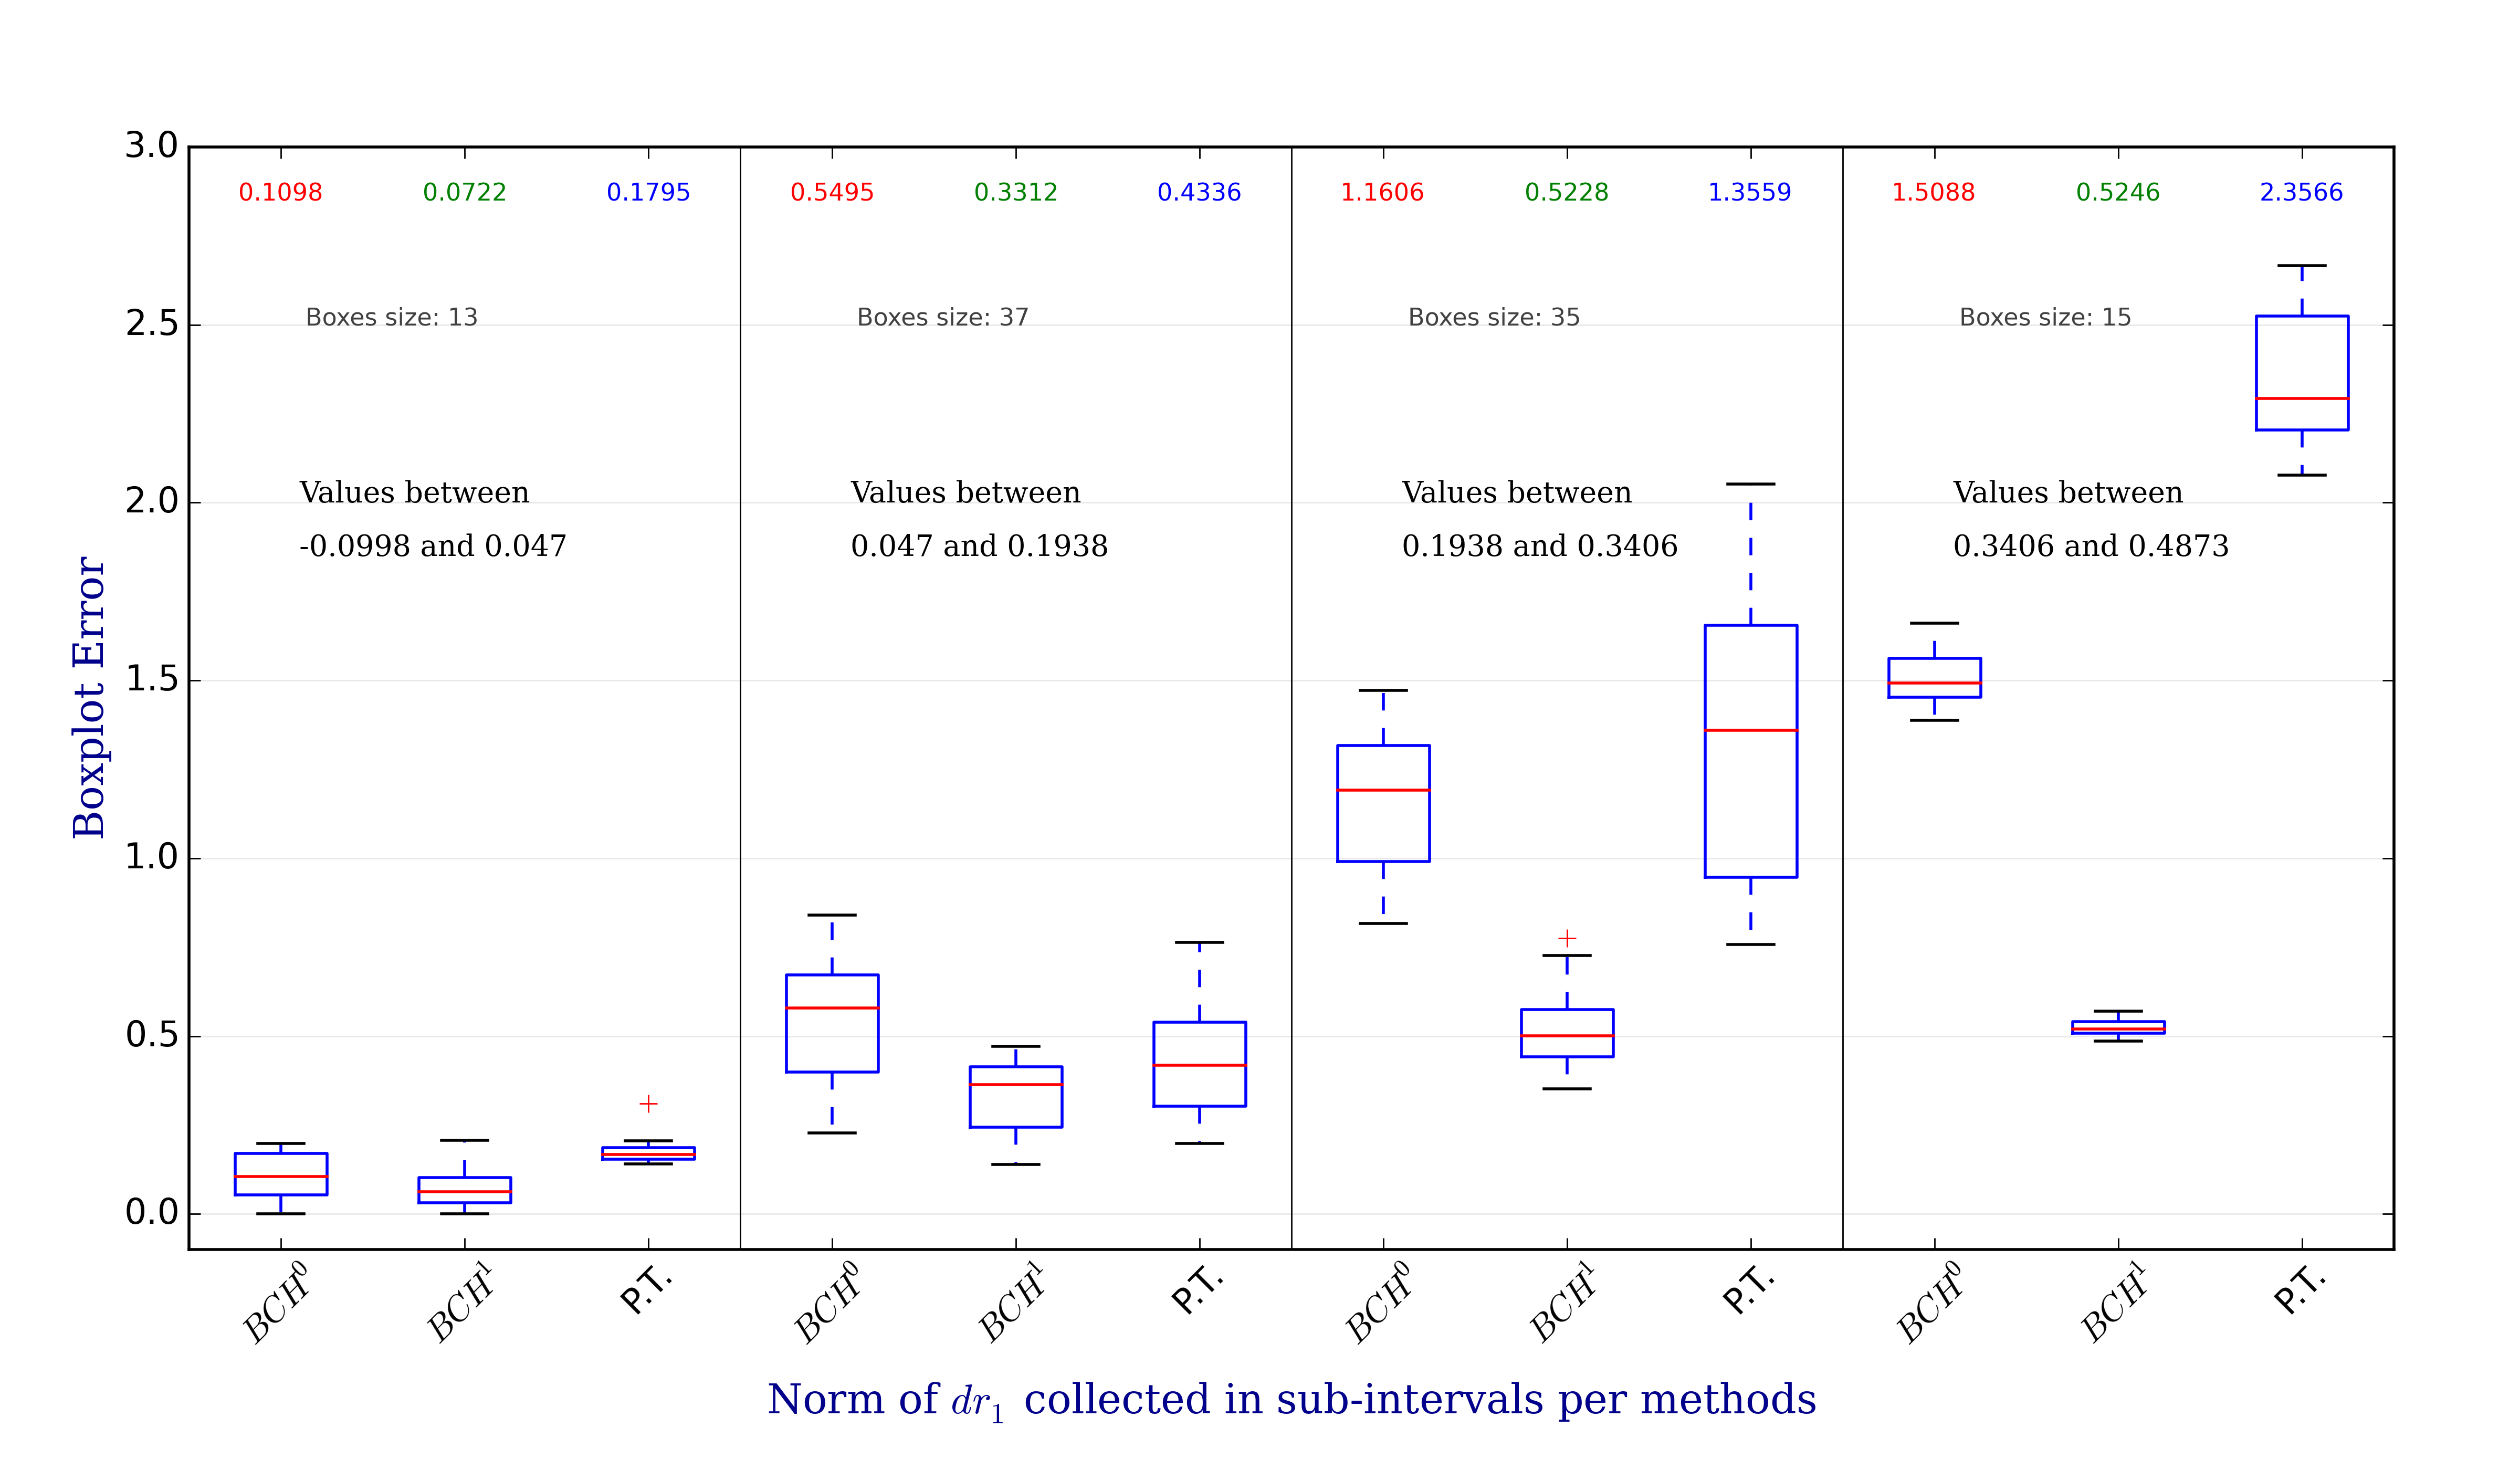
\includegraphics[scale=0.69]{figures/SVF_boxplot.png}
	\caption{Log-composition for SVF computed using numerical methods of truncated BCH of degree 0,1 and parallel transport, represented in a boxplot.}
	\label{fig:SVF_boxplot}
\end{figure}

\begin{figure}[!ht]
	\hspace{-2.5cm}
	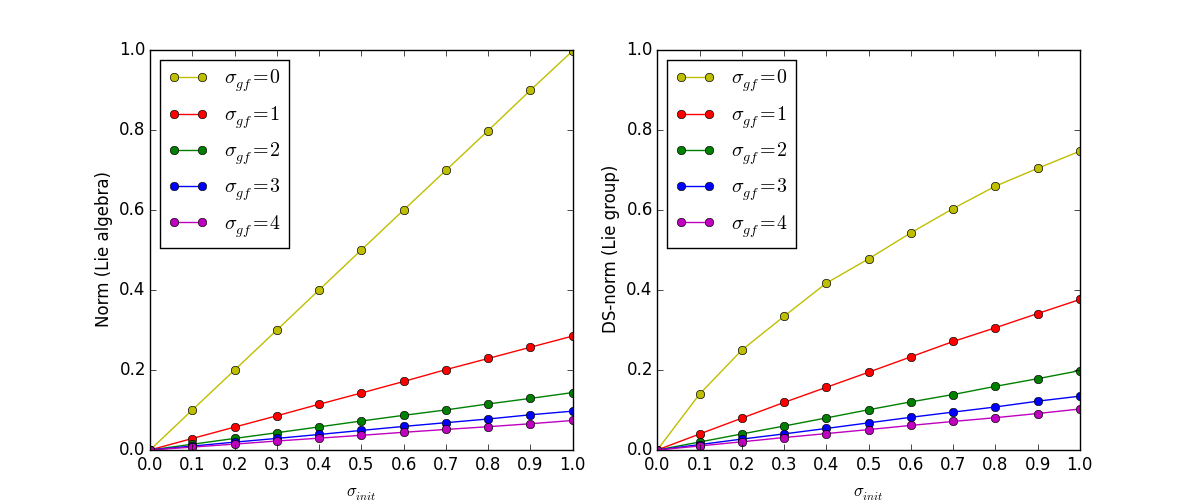
\includegraphics[scale=0.6]{figures/SVF_sigma_means_comparisons.png}
	\caption{Norm of random generated of SVF with initial standard deviation $\sigma_{\text{init}}$ (on the x-axis) and Gaussian filter with standard deviation $\sigma_{\text{gf}}$ (different colors). On the left is shown the the Frobenius norm computed on the SVF in the Lie algebra, while on the right the same norm is computed after the exponentiations. In this second case, the norm refers to the norm of the matrix data structure (DS-norm) utilized to parametrize the SVF. Each dot represents the mean of the norm of $10$ an SVF randomly generated with the parameters indicated on the axes and in the legend. We observe that the exponential bend the shape of the random SVF when the Gaussian filter is $0$ (thus we talk about an improper SVF). The decrease in the slope when $\sigma_{\text{gf}}=0$ do not appears for any other value.}
	\label{fig:SVF_sigma_means_comparisons}
\end{figure}





\begin{figure}[!ht]
	\hspace{-2.1cm}
	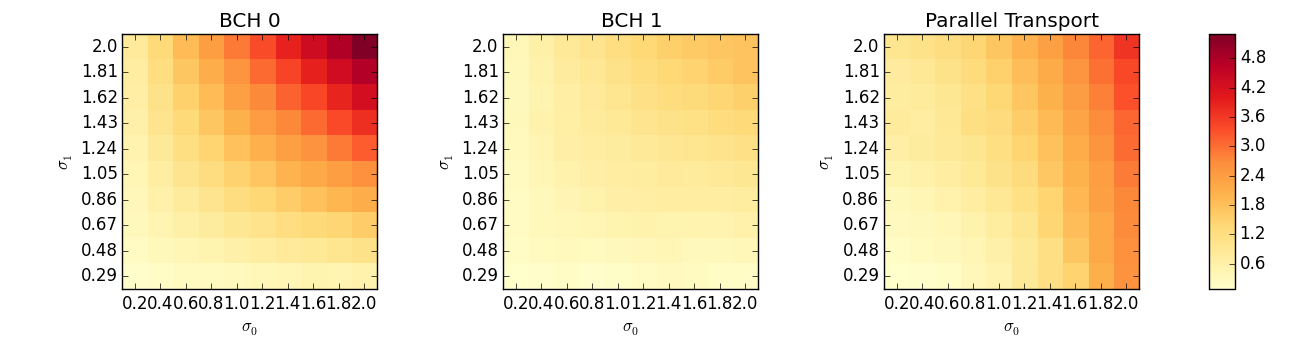
\includegraphics[scale=0.53]{figures/SVF_image_scale.png}
	\caption{Log-composition for SVF; the operation $\mathbf{u}_0\oplus \mathbf{u}_1$ is computed using numerical methods of truncated BCH of degree 0,1 and parallel transport. Respective standard deviation of the random generated SVF given by $\sigma_0$ and $\sigma_1$, ranges between $0.3$ and $2.0$ for $\sigma_0$ and between $0.2$ and $2.0$ for $\sigma_1$. Each value in the image scale is the mean of $10$ results of the log-computation of random SVF generated with given standard deviation. For lower values of $\mathbf{u}_1$, that in the image registration algorithms are given by the update, parallel transport method and truncated BCH of degree 1 have comparable results. We can also notice that for truncated BCH methods the results are symmetric, while for parallel transport, as expected from the formula, results are not symmetric respect to the size of the input vectors. }
	\label{fig:SVF_image_scale}
\end{figure}


% % % % % % % % % % % % % % % % % % % % % % % % % % % % % % % % % % % % % %
% % % % % % % % % % % % % % % % % % % % % % % % % % % % % % % % % % % % % % 
\subsection{Results}

% % % % % % % % % % % % % % % % % % % % % % % % % % % % % % % % % % % % % %
% % % % % % % % % % % % % % % % % % % % % % % % % % % % % % % % % % % % % % 
\subsection{Empirical Evaluations of Computational Time}

% % % % % % % % % % % % % % % % % % % % % % % % % % % % % % % % % % % % % %
% % % % % % % % % % % % % % % % % % % % % % % % % % % % % % % % % % % % % % 
% % % % % % % % % % % % % % % % % % % % % % % % % % % % % % % % % % % % % % 
\section{Log-Algorithm for SVF}

% % % % % % % % % % % % % % % % % % % % % % % % % % % % % % % % % % % % % %
% % % % % % % % % % % % % % % % % % % % % % % % % % % % % % % % % % % % % % 
\subsection{Methods}

% % % % % % % % % % % % % % % % % % % % % % % % % % % % % % % % % % % % % %
% % % % % % % % % % % % % % % % % % % % % % % % % % % % % % % % % % % % % % 
\subsection{Results}


% % % % % % % % % % % % % % % % % % % % % % % % % % % % % % % % % % % % % %
% % % % % % % % % % % % % % % % % % % % % % % % % % % % % % % % % % % % % % 
\subsection{Empirical Evaluations of Computational Time}


% % % % % % % % % % % % % % % % % % % % % % % % % % % % % % % % % % % % % %
% % % % % % % % % % % % % % % % % % % % % % % % % % % % % % % % % % % % % %
% % % % % % % % % % % % % % % % % % % % % % % % % % % % % % % % % % % % % % 
\section{Conclusions and Further Research}\label{ch:conclusions}


Considering only the results, this one-year research can be considered much ado about nothing, but...\\
Computational time...!

Starting from the definition of Lie log-group of diffeomorpshisms $(\mathfrak{g} , \oplus)$, to have an algebraic definition of this approximation, we can consider its quotient over the ideal generated by $(\text{ad}_{\mathbf{u}}^{m}, \text{ad}_{\mathbf{u}}^{n})$, which provides the group $(\quotient{\mathfrak{g}}{(\text{ad}_{\mathbf{u}}^{m}, \text{ad}_{\mathbf{u}}^{n})}, \oplus)$. Further investigations in this direction is not prosecuted.
